%% CHI submission template (acmart, sigconf format).
%% The 'review' option enables line numbers for reviewers.
%% The 'anonymous' option is intentionally omitted so author identity is shown.
\documentclass[sigconf,review]{acmart}

%%
%% \BibTeX command to typeset BibTeX logo in the docs
\AtBeginDocument{%
  \providecommand\BibTeX{{%
    Bib\TeX}}}

%% Submission metadata (paper not yet published; placeholders kept for production).
\setcopyright{none}
\copyrightyear{2026}
\acmYear{2026}
\acmConference[CHI '26]{Proceedings of the 2026 CHI Conference on Human Factors in Computing Systems}{April 13--17, 2026}{Barcelona, Spain}
\acmBooktitle{Proceedings of the 2026 CHI Conference on Human Factors in Computing Systems (CHI '26), April 13--17, 2026, Barcelona, Spain}

\usepackage{booktabs} % For formal tables
\usepackage{graphicx}
\usepackage{subcaption}
\usepackage{amsmath}
\usepackage{algorithm}
\usepackage{algpseudocode}

\begin{document}

\title{Performance Analysis of 3D Mesh Simplification Algorithms: QEM vs. Vertex Clustering on CAD and Organic Models}

\author{Ahnaf An Nafee}
\affiliation{%
  \institution{George Mason University}
  \city{Fairfax}
  \state{Virginia}
  \country{USA}
}
\email{aannafee@gmu.edu}

\begin{abstract}
High-fidelity 3D models often exceed the rendering budgets of real-time applications, necessitating effective mesh simplification algorithms. However, current benchmarks often overlook the impact of input mesh topology, specifically the distinction between structured CAD models and unstructured organic scans. This paper presents a comparative analysis of two fundamental simplification algorithms: Quadric Error Metrics (QEM) and Vertex Clustering. We evaluate these algorithms across two distinct datasets (ModelNet40 for CAD and Thingi10K for Organic models) at varying levels of decimation (50\% and 90\%). Using a rigorous factorial experimental design, we quantify Execution Time and Geometric Fidelity (Hausdorff Distance). We demonstrate that Vertex Clustering is orders of magnitude faster ($p < 0.001$) and remarkably stable across all datasets. Conversely, while QEM offers superior accuracy at moderate reduction levels, we identify a significant performance degradation on organic meshes and a catastrophic loss of geometric fidelity on sparse CAD models at high decimation levels. Our findings establish that the optimal choice of simplification strategy depends heavily on the source topology and the target decimation ratio.
\end{abstract}

\begin{CCSXML}
<ccs2012>
   <concept>
       <concept_id>10010147.10010371.10010396.10010398</concept_id>
       <concept_desc>Computing methodologies~Mesh geometry models</concept_desc>
       <concept_significance>500</concept_significance>
       </concept>
   <concept>
       <concept_id>10002950.10003714.10003715.10003705</concept_id>
       <concept_desc>Mathematics of computing~Geometric topology</concept_desc>
       <concept_significance>300</concept_significance>
       </concept>
 </ccs2012>
\end{CCSXML}

\ccsdesc[500]{Computing methodologies~Mesh geometry models}
\ccsdesc[300]{Mathematics of computing~Geometric topology}

\keywords{Mesh Simplification, Level of Detail, Performance Analysis, Quadric Error Metrics, Vertex Clustering}

\maketitle

\begin{figure*}[t]
  \centering
  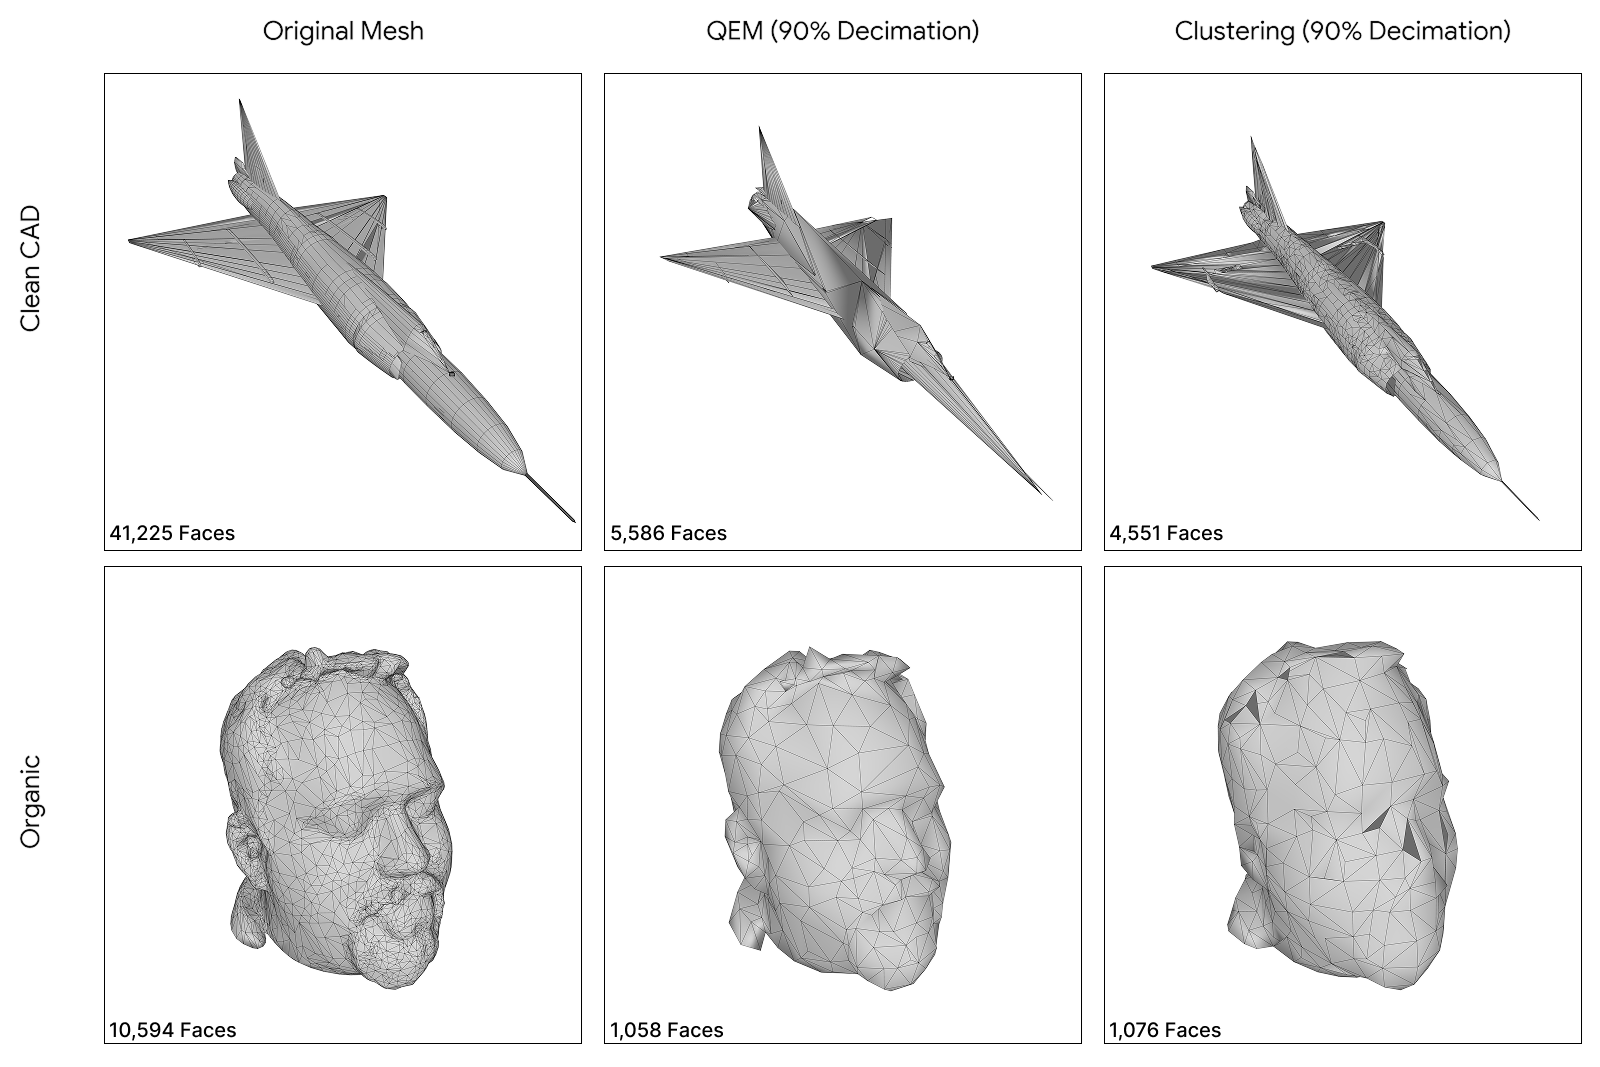
\includegraphics[width=0.95\textwidth]{figures/teaser.png}
  \caption{Visual comparison of decimation stability at \textbf{90\% target reduction}. \textbf{Top Row (Clean CAD - Airplane, 33k Faces):} QEM (center) suffers from catastrophic topological collapse, destroying the wings and fuselage. Vertex Clustering (right) produces a coarse approximation but preserves global connectivity. \textbf{Bottom Row (Organic - Face, 10.5k Faces):} QEM excels at preserving smooth curvature, whereas Clustering introduces uniform geometric aliasing.}
  \Description{Comparison of QEM and Clustering algorithms on Airplane (CAD) and Face (Organic) models. QEM fails on the airplane, removing wings, while Clustering keeps the shape but is blocky. Both work well on the face, but QEM is smoother.}
  \label{fig:teaser}
\end{figure*}

\input{sections/introduction}
\input{sections/related-work}
\input{sections/problem-description}
\input{sections/methodology}
\input{sections/results}
\input{sections/discussion}
\input{sections/future-work}
\input{sections/conclusion}

\end{document}
